\documentclass[mode=tex]{standalone}
% \usepackage{pgfplots}
% \pgfplotsset{width=\linewidth,compat=3.1.10}
% \usepackage{pgfplotstable}
\usepackage{amsfonts}
\usepackage{amsmath}
\usepackage{tikz}
\usetikzlibrary{arrows.meta}
\begin{document}

% \begin{tikzpicture}
% \draw [<->, thick, -{Stealth[round]}] (-1, -1) -- (-1, 1); 
% \draw [<->, thick, -{Stealth[round]}] (1, -1) -- (1, 1);
% \draw [dotted, thick] (-1, 1) -- (1, 1);
% \draw [dotted, thick] (-1, -1) -- (1, -1);
% % top left
% \draw [->, thick, -{Stealth[round]}] (-1, 1) -- (-1.3, 1.4);
% \draw [->, thick, -{Stealth[round]}] (-1, 1) -- (-0.7, 1.4);
% % top right 
% \draw [->, thick, -{Stealth[round]}] (1, 1) -- (1.3, 1.4);
% \draw [->, thick, -{Stealth[round]}] (1, 1) -- (0.7, 1.4);
% % bottom left
% \draw [->, thick, -{Stealth[round]}] (-1, -1) -- (-1.3, -1.4);
% \draw [->, thick, -{Stealth[round]}] (-1, -1) -- (-0.7, -1.4);
% % bottom right 
% \draw [->, thick, -{Stealth[round]}] (1, -1) -- (1.3, -1.4);
% \draw [->, thick, -{Stealth[round]}] (1, -1) -- (0.7, -1.4);
% \end{tikzpicture}

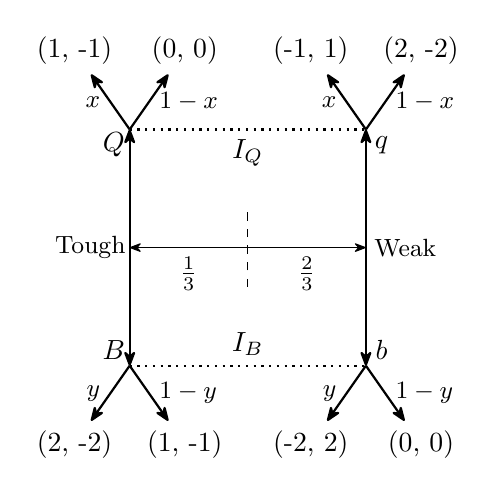
\begin{tikzpicture}[>={Stealth[round]}]
    \node (Q) at (-1.2-0.5, 1-0.2 + 0.5) {$Q$};
    % \node (Quiche) at (-1.7, 1.1) {\small{Quiche}};
    % \node (Beer) at (-1.7, -1.1) {\small{Beer}};
    \node (q) at (1.2+0.5, 1-0.2+0.5) {$q$};
    \node (B) at (-1.2-0.5, -1+0.2-0.5) {$B$};
    \node (b) at (1.2+0.5, -1+0.2-0.5) {$b$};
    \node [coordinate](QB) at (-1-0.5, 0) {};
    \node [coordinate](qb) at (1+0.5, 0) {};
    \path[->] (0, 0) edge node[below] {$\frac{1}{3}$}  (QB);
    \path[->] (0, 0) edge node[below] {$\frac{2}{3}$}  (qb);
    \draw [<->, thick] (-1-0.5, -1-0.5) -- (-1-0.5, 1+0.5); 
    \draw [<->, thick] (1+0.5, -1-0.5) -- (1+0.5, 1+0.5);
    \path [dotted, thick] (-1-0.5, 1+0.5) edge node[below] {$I_Q$} (1.5, 1.5);
    \path [dotted, thick] (-1.5, -1.5) edge node[above] {$I_B$} (1.5, -1.5);
    \node (T) at (-2, 0) {\small{Tough}};
    \node (W) at (2, 0) {\small{Weak}};
    \node (p1) at (-2.2, 2.5) {(1, -1)};
    \node (p2) at (-0.8, 2.5) {(0, 0)};
    \path [->, thick] (-1.5, 1.5) edge node[below, left] {\small{$x$}} (p1);
    \path [->, thick] (-1.5, 1.5) edge node[below, right] {\small{$1-x$}} (p2);

    \node (p3) at (0.8, 2.5) {(-1, 1)};
    \node (p4) at (2.2, 2.5) {(2, -2)};
    \path [->, thick] (1.5, 1.5) edge node[below, left] {\small{$x$}} (p3);
    \path [->, thick] (1.5, 1.5) edge node[below, right] {\small{$1-x$}} (p4);

    
    \node (p5) at (-2.2, -2.5) {(2, -2)};
    \node (p6) at (-0.8, -2.5) {(1, -1)};
    \path [->, thick] (-1.5, -1.5) edge node[below, left] {\small{$y$}} (p5);
    \path [->, thick] (-1.5, -1.5) edge node[below, right] {\small{$1-y$}} (p6);

    
    \node (p7) at (0.8, -2.5) {(-2, 2)};
    \node (p8) at (2.2, -2.5) {(0, 0)};
    \path [->, thick] (1.5, -1.5) edge node[below, left] {\small{$y$}} (p7);
    \path [->, thick] (1.5, -1.5) edge node[below, right] {\small{$1-y$}} (p8);
    % \path [->, thick] (-1, 1) edge node[below left] {$x$} (-1.4, 1.5);
    % \draw [->, thick, -{Stealth[round]}] (-1, 1) -- (-0.7, 1.4);
    % % top right 
    % \draw [->, thick, -{Stealth[round]}] (1, 1) -- (1.3, 1.4);
    % \draw [->, thick, -{Stealth[round]}] (1, 1) -- (0.7, 1.4);
    % % bottom left
    % \draw [->, thick, -{Stealth[round]}] (-1, -1) -- (-1.3, -1.4);
    % \draw [->, thick, -{Stealth[round]}] (-1, -1) -- (-0.7, -1.4);
    % % bottom right 
    % \draw [->, thick, -{Stealth[round]}] (1, -1) -- (1.3, -1.4);
    % \draw [->, thick, -{Stealth[round]}] (1, -1) -- (0.7, -1.4);


    \draw [dashed] (0, -0.5) -- (0, 0.5);

\end{tikzpicture}
\end{document}